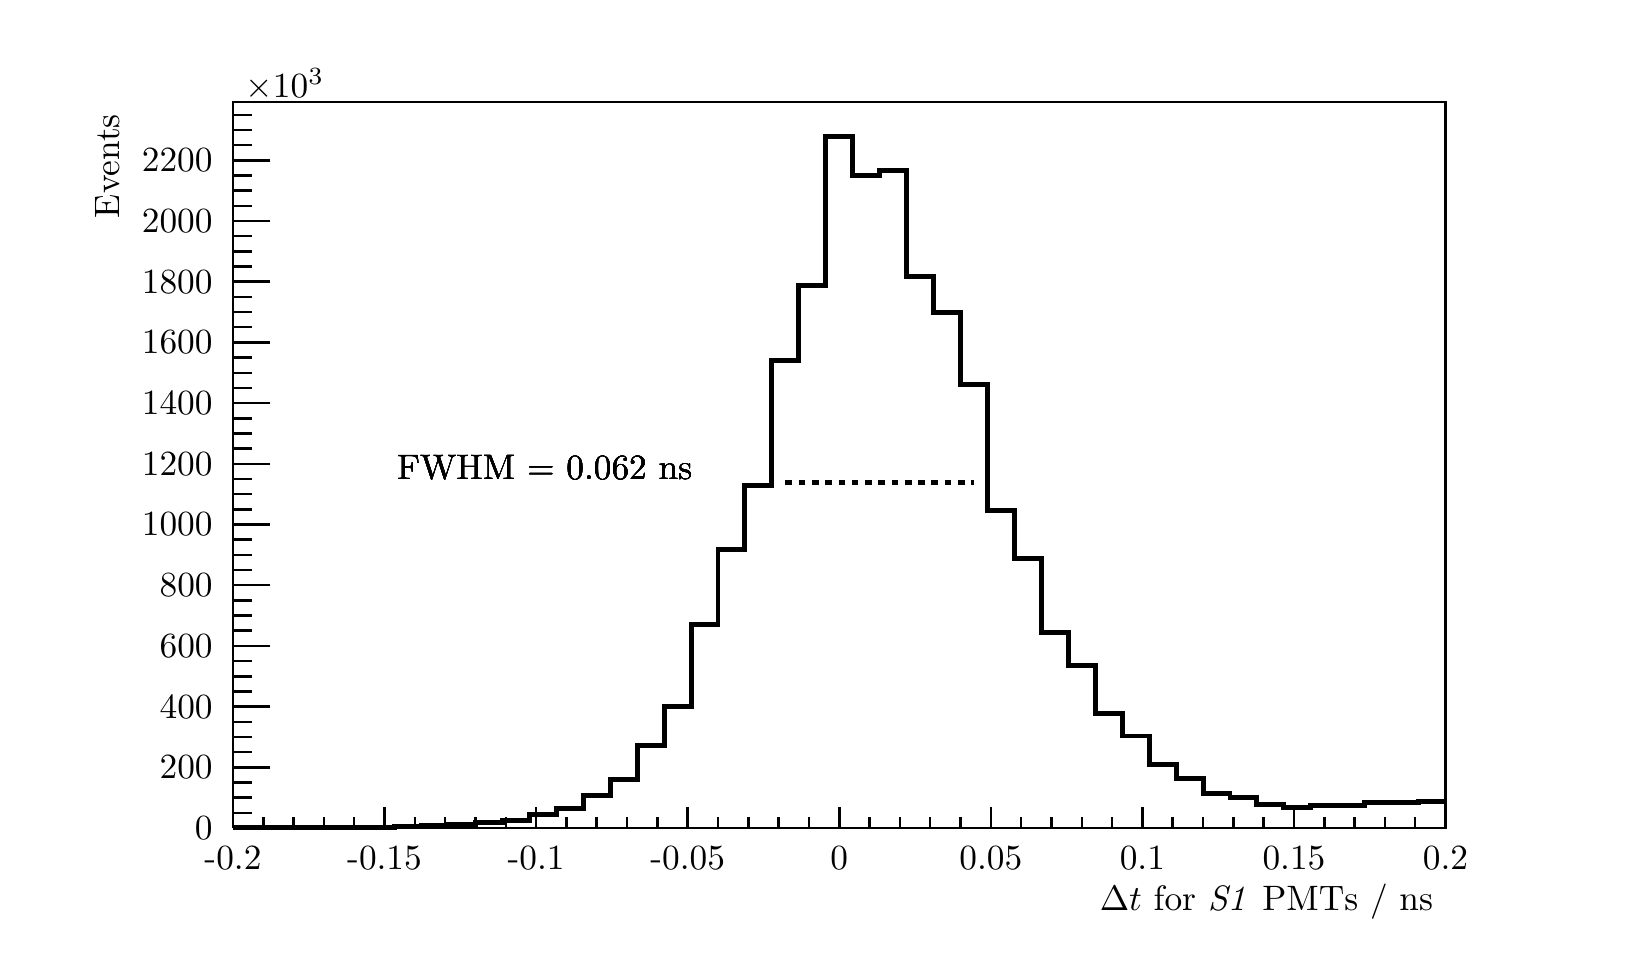
\begin{tikzpicture}
\pgfdeclareplotmark{cross} {
\pgfpathmoveto{\pgfpoint{-0.3\pgfplotmarksize}{\pgfplotmarksize}}
\pgfpathlineto{\pgfpoint{+0.3\pgfplotmarksize}{\pgfplotmarksize}}
\pgfpathlineto{\pgfpoint{+0.3\pgfplotmarksize}{0.3\pgfplotmarksize}}
\pgfpathlineto{\pgfpoint{+1\pgfplotmarksize}{0.3\pgfplotmarksize}}
\pgfpathlineto{\pgfpoint{+1\pgfplotmarksize}{-0.3\pgfplotmarksize}}
\pgfpathlineto{\pgfpoint{+0.3\pgfplotmarksize}{-0.3\pgfplotmarksize}}
\pgfpathlineto{\pgfpoint{+0.3\pgfplotmarksize}{-1.\pgfplotmarksize}}
\pgfpathlineto{\pgfpoint{-0.3\pgfplotmarksize}{-1.\pgfplotmarksize}}
\pgfpathlineto{\pgfpoint{-0.3\pgfplotmarksize}{-0.3\pgfplotmarksize}}
\pgfpathlineto{\pgfpoint{-1.\pgfplotmarksize}{-0.3\pgfplotmarksize}}
\pgfpathlineto{\pgfpoint{-1.\pgfplotmarksize}{0.3\pgfplotmarksize}}
\pgfpathlineto{\pgfpoint{-0.3\pgfplotmarksize}{0.3\pgfplotmarksize}}
\pgfpathclose
\pgfusepathqstroke
}
\pgfdeclareplotmark{cross*} {
\pgfpathmoveto{\pgfpoint{-0.3\pgfplotmarksize}{\pgfplotmarksize}}
\pgfpathlineto{\pgfpoint{+0.3\pgfplotmarksize}{\pgfplotmarksize}}
\pgfpathlineto{\pgfpoint{+0.3\pgfplotmarksize}{0.3\pgfplotmarksize}}
\pgfpathlineto{\pgfpoint{+1\pgfplotmarksize}{0.3\pgfplotmarksize}}
\pgfpathlineto{\pgfpoint{+1\pgfplotmarksize}{-0.3\pgfplotmarksize}}
\pgfpathlineto{\pgfpoint{+0.3\pgfplotmarksize}{-0.3\pgfplotmarksize}}
\pgfpathlineto{\pgfpoint{+0.3\pgfplotmarksize}{-1.\pgfplotmarksize}}
\pgfpathlineto{\pgfpoint{-0.3\pgfplotmarksize}{-1.\pgfplotmarksize}}
\pgfpathlineto{\pgfpoint{-0.3\pgfplotmarksize}{-0.3\pgfplotmarksize}}
\pgfpathlineto{\pgfpoint{-1.\pgfplotmarksize}{-0.3\pgfplotmarksize}}
\pgfpathlineto{\pgfpoint{-1.\pgfplotmarksize}{0.3\pgfplotmarksize}}
\pgfpathlineto{\pgfpoint{-0.3\pgfplotmarksize}{0.3\pgfplotmarksize}}
\pgfpathclose
\pgfusepathqfillstroke
}
\pgfdeclareplotmark{newstar} {
\pgfpathmoveto{\pgfqpoint{0pt}{\pgfplotmarksize}}
\pgfpathlineto{\pgfqpointpolar{44}{0.5\pgfplotmarksize}}
\pgfpathlineto{\pgfqpointpolar{18}{\pgfplotmarksize}}
\pgfpathlineto{\pgfqpointpolar{-20}{0.5\pgfplotmarksize}}
\pgfpathlineto{\pgfqpointpolar{-54}{\pgfplotmarksize}}
\pgfpathlineto{\pgfqpointpolar{-90}{0.5\pgfplotmarksize}}
\pgfpathlineto{\pgfqpointpolar{234}{\pgfplotmarksize}}
\pgfpathlineto{\pgfqpointpolar{198}{0.5\pgfplotmarksize}}
\pgfpathlineto{\pgfqpointpolar{162}{\pgfplotmarksize}}
\pgfpathlineto{\pgfqpointpolar{134}{0.5\pgfplotmarksize}}
\pgfpathclose
\pgfusepathqstroke
}
\pgfdeclareplotmark{newstar*} {
\pgfpathmoveto{\pgfqpoint{0pt}{\pgfplotmarksize}}
\pgfpathlineto{\pgfqpointpolar{44}{0.5\pgfplotmarksize}}
\pgfpathlineto{\pgfqpointpolar{18}{\pgfplotmarksize}}
\pgfpathlineto{\pgfqpointpolar{-20}{0.5\pgfplotmarksize}}
\pgfpathlineto{\pgfqpointpolar{-54}{\pgfplotmarksize}}
\pgfpathlineto{\pgfqpointpolar{-90}{0.5\pgfplotmarksize}}
\pgfpathlineto{\pgfqpointpolar{234}{\pgfplotmarksize}}
\pgfpathlineto{\pgfqpointpolar{198}{0.5\pgfplotmarksize}}
\pgfpathlineto{\pgfqpointpolar{162}{\pgfplotmarksize}}
\pgfpathlineto{\pgfqpointpolar{134}{0.5\pgfplotmarksize}}
\pgfpathclose
\pgfusepathqfillstroke
}
\definecolor{c}{rgb}{1,1,1};
\draw [color=c, fill=c] (0,0) rectangle (20,11.675);
\draw [color=c, fill=c] (2.6,1.51775) rectangle (18,10.741);
\definecolor{c}{rgb}{0,0,0};
\draw [c,line width=0.9] (2.6,1.51775) -- (2.6,10.741) -- (18,10.741) -- (18,1.51775) -- (2.6,1.51775);
\definecolor{c}{rgb}{1,1,1};
\draw [color=c, fill=c] (2.6,1.51775) rectangle (18,10.741);
\definecolor{c}{rgb}{0,0,0};
\draw [c,line width=0.9] (2.6,1.51775) -- (2.6,10.741) -- (18,10.741) -- (18,1.51775) -- (2.6,1.51775);
\draw [c,line width=1.8] (2.6,1.51958) -- (2.94222,1.51958) -- (2.94222,1.51977) -- (3.28444,1.51977) -- (3.28444,1.52075) -- (3.62667,1.52075) -- (3.62667,1.52204) -- (3.96889,1.52204) -- (3.96889,1.52504) -- (4.31111,1.52504) -- (4.31111,1.52834)
 -- (4.65333,1.52834) -- (4.65333,1.53523) -- (4.99556,1.53523) -- (4.99556,1.54741) -- (5.33778,1.54741) -- (5.33778,1.5584) -- (5.68,1.5584) -- (5.68,1.58483) -- (6.02222,1.58483) -- (6.02222,1.61641) -- (6.36444,1.61641) -- (6.36444,1.68501) --
 (6.70667,1.68501) -- (6.70667,1.76425) -- (7.04889,1.76425) -- (7.04889,1.93053) -- (7.39111,1.93053) -- (7.39111,2.12776) -- (7.73333,2.12776) -- (7.73333,2.57125) -- (8.07556,2.57125) -- (8.07556,3.05548) -- (8.41778,3.05548) -- (8.41778,4.09746)
 -- (8.76,4.09746) -- (8.76,5.05002) -- (9.10222,5.05002) -- (9.10222,5.87277) -- (9.44444,5.87277) -- (9.44444,7.45651) -- (9.78667,7.45651) -- (9.78667,8.4135) -- (10.1289,8.4135) -- (10.1289,10.3018) -- (10.4711,10.3018) -- (10.4711,9.8074) --
 (10.8133,9.8074) -- (10.8133,9.87378) -- (11.1556,9.87378) -- (11.1556,8.52277) -- (11.4978,8.52277) -- (11.4978,8.05893) -- (11.84,8.05893) -- (11.84,7.14883) -- (12.1822,7.14883) -- (12.1822,5.55186) -- (12.5244,5.55186) -- (12.5244,4.94574) --
 (12.8667,4.94574) -- (12.8667,3.99644) -- (13.2089,3.99644) -- (13.2089,3.57792) -- (13.5511,3.57792) -- (13.5511,2.9767) -- (13.8933,2.9767) -- (13.8933,2.68633) -- (14.2356,2.68633) -- (14.2356,2.31822) -- (14.5778,2.31822) -- (14.5778,2.15102) --
 (14.92,2.15102) -- (14.92,1.96062) -- (15.2622,1.96062) -- (15.2622,1.90122) -- (15.6044,1.90122) -- (15.6044,1.81479) -- (15.9467,1.81479) -- (15.9467,1.78186) -- (16.2889,1.78186) -- (16.2889,1.80117) -- (16.6311,1.80117) -- (16.6311,1.80069) --
 (16.9733,1.80069) -- (16.9733,1.8367) -- (17.3156,1.8367) -- (17.3156,1.83646) -- (17.6578,1.83646) -- (17.6578,1.84969) -- (18,1.84969);
\draw [c,line width=0.9] (2.6,1.51775) -- (18,1.51775);
\draw [c,line width=0.9] (2.6,1.78744) -- (2.6,1.51775);
\draw [c,line width=0.9] (2.985,1.6526) -- (2.985,1.51775);
\draw [c,line width=0.9] (3.37,1.6526) -- (3.37,1.51775);
\draw [c,line width=0.9] (3.755,1.6526) -- (3.755,1.51775);
\draw [c,line width=0.9] (4.14,1.6526) -- (4.14,1.51775);
\draw [c,line width=0.9] (4.525,1.78744) -- (4.525,1.51775);
\draw [c,line width=0.9] (4.91,1.6526) -- (4.91,1.51775);
\draw [c,line width=0.9] (5.295,1.6526) -- (5.295,1.51775);
\draw [c,line width=0.9] (5.68,1.6526) -- (5.68,1.51775);
\draw [c,line width=0.9] (6.065,1.6526) -- (6.065,1.51775);
\draw [c,line width=0.9] (6.45,1.78744) -- (6.45,1.51775);
\draw [c,line width=0.9] (6.835,1.6526) -- (6.835,1.51775);
\draw [c,line width=0.9] (7.22,1.6526) -- (7.22,1.51775);
\draw [c,line width=0.9] (7.605,1.6526) -- (7.605,1.51775);
\draw [c,line width=0.9] (7.99,1.6526) -- (7.99,1.51775);
\draw [c,line width=0.9] (8.375,1.78744) -- (8.375,1.51775);
\draw [c,line width=0.9] (8.76,1.6526) -- (8.76,1.51775);
\draw [c,line width=0.9] (9.145,1.6526) -- (9.145,1.51775);
\draw [c,line width=0.9] (9.53,1.6526) -- (9.53,1.51775);
\draw [c,line width=0.9] (9.915,1.6526) -- (9.915,1.51775);
\draw [c,line width=0.9] (10.3,1.78744) -- (10.3,1.51775);
\draw [c,line width=0.9] (10.685,1.6526) -- (10.685,1.51775);
\draw [c,line width=0.9] (11.07,1.6526) -- (11.07,1.51775);
\draw [c,line width=0.9] (11.455,1.6526) -- (11.455,1.51775);
\draw [c,line width=0.9] (11.84,1.6526) -- (11.84,1.51775);
\draw [c,line width=0.9] (12.225,1.78744) -- (12.225,1.51775);
\draw [c,line width=0.9] (12.61,1.6526) -- (12.61,1.51775);
\draw [c,line width=0.9] (12.995,1.6526) -- (12.995,1.51775);
\draw [c,line width=0.9] (13.38,1.6526) -- (13.38,1.51775);
\draw [c,line width=0.9] (13.765,1.6526) -- (13.765,1.51775);
\draw [c,line width=0.9] (14.15,1.78744) -- (14.15,1.51775);
\draw [c,line width=0.9] (14.535,1.6526) -- (14.535,1.51775);
\draw [c,line width=0.9] (14.92,1.6526) -- (14.92,1.51775);
\draw [c,line width=0.9] (15.305,1.6526) -- (15.305,1.51775);
\draw [c,line width=0.9] (15.69,1.6526) -- (15.69,1.51775);
\draw [c,line width=0.9] (16.075,1.78744) -- (16.075,1.51775);
\draw [c,line width=0.9] (16.46,1.6526) -- (16.46,1.51775);
\draw [c,line width=0.9] (16.845,1.6526) -- (16.845,1.51775);
\draw [c,line width=0.9] (17.23,1.6526) -- (17.23,1.51775);
\draw [c,line width=0.9] (17.615,1.6526) -- (17.615,1.51775);
\draw [c,line width=0.9] (18,1.78744) -- (18,1.51775);
\draw [anchor=base] (2.6,0.992375) node[scale=1.27706, color=c, rotate=0]{-0.2};
\draw [anchor=base] (4.525,0.992375) node[scale=1.27706, color=c, rotate=0]{-0.15};
\draw [anchor=base] (6.45,0.992375) node[scale=1.27706, color=c, rotate=0]{-0.1};
\draw [anchor=base] (8.375,0.992375) node[scale=1.27706, color=c, rotate=0]{-0.05};
\draw [anchor=base] (10.3,0.992375) node[scale=1.27706, color=c, rotate=0]{0};
\draw [anchor=base] (12.225,0.992375) node[scale=1.27706, color=c, rotate=0]{0.05};
\draw [anchor=base] (14.15,0.992375) node[scale=1.27706, color=c, rotate=0]{0.1};
\draw [anchor=base] (16.075,0.992375) node[scale=1.27706, color=c, rotate=0]{0.15};
\draw [anchor=base] (18,0.992375) node[scale=1.27706, color=c, rotate=0]{0.2};
\draw [anchor= east] (18,0.58375) node[scale=1.27706, color=c, rotate=0]{$\Delta t$ for $\mathit{S1}$ PMTs / ns};
\draw [c,line width=0.9] (2.6,1.51775) -- (2.6,10.741);
\draw [c,line width=0.9] (3.074,1.51775) -- (2.6,1.51775);
\draw [c,line width=0.9] (2.837,1.71046) -- (2.6,1.71046);
\draw [c,line width=0.9] (2.837,1.90318) -- (2.6,1.90318);
\draw [c,line width=0.9] (2.837,2.09589) -- (2.6,2.09589);
\draw [c,line width=0.9] (3.074,2.2886) -- (2.6,2.2886);
\draw [c,line width=0.9] (2.837,2.48132) -- (2.6,2.48132);
\draw [c,line width=0.9] (2.837,2.67403) -- (2.6,2.67403);
\draw [c,line width=0.9] (2.837,2.86674) -- (2.6,2.86674);
\draw [c,line width=0.9] (3.074,3.05946) -- (2.6,3.05946);
\draw [c,line width=0.9] (2.837,3.25217) -- (2.6,3.25217);
\draw [c,line width=0.9] (2.837,3.44488) -- (2.6,3.44488);
\draw [c,line width=0.9] (2.837,3.6376) -- (2.6,3.6376);
\draw [c,line width=0.9] (3.074,3.83031) -- (2.6,3.83031);
\draw [c,line width=0.9] (2.837,4.02302) -- (2.6,4.02302);
\draw [c,line width=0.9] (2.837,4.21574) -- (2.6,4.21574);
\draw [c,line width=0.9] (2.837,4.40845) -- (2.6,4.40845);
\draw [c,line width=0.9] (3.074,4.60116) -- (2.6,4.60116);
\draw [c,line width=0.9] (2.837,4.79388) -- (2.6,4.79388);
\draw [c,line width=0.9] (2.837,4.98659) -- (2.6,4.98659);
\draw [c,line width=0.9] (2.837,5.1793) -- (2.6,5.1793);
\draw [c,line width=0.9] (3.074,5.37202) -- (2.6,5.37202);
\draw [c,line width=0.9] (2.837,5.56473) -- (2.6,5.56473);
\draw [c,line width=0.9] (2.837,5.75744) -- (2.6,5.75744);
\draw [c,line width=0.9] (2.837,5.95016) -- (2.6,5.95016);
\draw [c,line width=0.9] (3.074,6.14287) -- (2.6,6.14287);
\draw [c,line width=0.9] (2.837,6.33558) -- (2.6,6.33558);
\draw [c,line width=0.9] (2.837,6.5283) -- (2.6,6.5283);
\draw [c,line width=0.9] (2.837,6.72101) -- (2.6,6.72101);
\draw [c,line width=0.9] (3.074,6.91372) -- (2.6,6.91372);
\draw [c,line width=0.9] (2.837,7.10644) -- (2.6,7.10644);
\draw [c,line width=0.9] (2.837,7.29915) -- (2.6,7.29915);
\draw [c,line width=0.9] (2.837,7.49186) -- (2.6,7.49186);
\draw [c,line width=0.9] (3.074,7.68458) -- (2.6,7.68458);
\draw [c,line width=0.9] (2.837,7.87729) -- (2.6,7.87729);
\draw [c,line width=0.9] (2.837,8.07) -- (2.6,8.07);
\draw [c,line width=0.9] (2.837,8.26272) -- (2.6,8.26272);
\draw [c,line width=0.9] (3.074,8.45543) -- (2.6,8.45543);
\draw [c,line width=0.9] (2.837,8.64814) -- (2.6,8.64814);
\draw [c,line width=0.9] (2.837,8.84086) -- (2.6,8.84086);
\draw [c,line width=0.9] (2.837,9.03357) -- (2.6,9.03357);
\draw [c,line width=0.9] (3.074,9.22628) -- (2.6,9.22628);
\draw [c,line width=0.9] (2.837,9.419) -- (2.6,9.419);
\draw [c,line width=0.9] (2.837,9.61171) -- (2.6,9.61171);
\draw [c,line width=0.9] (2.837,9.80442) -- (2.6,9.80442);
\draw [c,line width=0.9] (3.074,9.99714) -- (2.6,9.99714);
\draw [c,line width=0.9] (3.074,9.99714) -- (2.6,9.99714);
\draw [c,line width=0.9] (2.837,10.1899) -- (2.6,10.1899);
\draw [c,line width=0.9] (2.837,10.3826) -- (2.6,10.3826);
\draw [c,line width=0.9] (2.837,10.5753) -- (2.6,10.5753);
\draw [anchor= east] (2.5,1.51775) node[scale=1.27706, color=c, rotate=0]{0};
\draw [anchor= east] (2.5,2.2886) node[scale=1.27706, color=c, rotate=0]{200};
\draw [anchor= east] (2.5,3.05946) node[scale=1.27706, color=c, rotate=0]{400};
\draw [anchor= east] (2.5,3.83031) node[scale=1.27706, color=c, rotate=0]{600};
\draw [anchor= east] (2.5,4.60116) node[scale=1.27706, color=c, rotate=0]{800};
\draw [anchor= east] (2.5,5.37202) node[scale=1.27706, color=c, rotate=0]{1000};
\draw [anchor= east] (2.5,6.14287) node[scale=1.27706, color=c, rotate=0]{1200};
\draw [anchor= east] (2.5,6.91372) node[scale=1.27706, color=c, rotate=0]{1400};
\draw [anchor= east] (2.5,7.68458) node[scale=1.27706, color=c, rotate=0]{1600};
\draw [anchor= east] (2.5,8.45543) node[scale=1.27706, color=c, rotate=0]{1800};
\draw [anchor= east] (2.5,9.22628) node[scale=1.27706, color=c, rotate=0]{2000};
\draw [anchor= east] (2.5,9.99714) node[scale=1.27706, color=c, rotate=0]{2200};
\draw [anchor=base west] (2.6,10.7994) node[scale=1.27706, color=c, rotate=0]{$\times10^{3}$};
\draw [anchor= east] (1,10.741) node[scale=1.27706, color=c, rotate=90]{ Events};
\draw [c,dash pattern=on 2.40pt off 2.40pt ,line width=1.8] (9.61556,5.90977) -- (12.0111,5.90977);
\draw [anchor=base west] (4.525,5.95016) node[scale=1.27706, color=c, rotate=0]{FWHM = 0.062 ns};
\draw [anchor=base west] (4.525,5.95016) node[scale=1.27706, color=c, rotate=0]{FWHM = 0.062 ns};
\draw [anchor=base west] (4.525,5.95016) node[scale=1.27706, color=c, rotate=0]{FWHM = 0.062 ns};
\draw [anchor=base west] (4.525,5.95016) node[scale=1.27706, color=c, rotate=0]{FWHM = 0.062 ns};
\draw [anchor=base west] (4.525,5.95016) node[scale=1.27706, color=c, rotate=0]{FWHM = 0.062 ns};
\end{tikzpicture}
